\documentclass[aspectratio=169]{beamer}

% Theme Setup
\usetheme{Madrid}
\usecolortheme{beaver} % Red theme

% Packages
\usepackage{graphicx}
\usepackage{tikz}
\usetikzlibrary{shapes, arrows, positioning}
\usepackage{listings}
\usepackage{xcolor}
\usepackage{hyperref}
\usepackage{booktabs}

% TikZ Setup for Flowcharts
\tikzstyle{block} = [rectangle, draw, fill=red!20,
    text width=5em, text centered, rounded corners, minimum height=3em]
\tikzstyle{line} = [draw, -latex']

% Code Listing Setup
\lstset{
    language=Python,
    basicstyle=\ttfamily\small,
    keywordstyle=\color{blue},
    stringstyle=\color{red},
    commentstyle=\color{green!60!black},
    showstringspaces=false,
    breaklines=true,
    frame=single
}

% Title Info
\title{Introduction to Reinforcement Learning}
\subtitle{From Fundamentals to Flappy Bird}
\author{CPCS-331 Workshop Team}
\institute{KAUST Academy AI Summer School Alumni}
\date{\today}

\begin{document}

% -----------------------------------------------------------------------------
% Slide 1: Title
% -----------------------------------------------------------------------------
\begin{frame}
    \titlepage
\end{frame}

% -----------------------------------------------------------------------------
% Section 1: Introduction
% -----------------------------------------------------------------------------
\section{Introduction}

\begin{frame}
    \frametitle{The Hook}
    \begin{columns}
        \column{0.5\textwidth}
        \centering
        \textbf{What if machines could learn like us?}
        \vspace{1cm}

        \textit{"No manual. No map. Just trial and error."}

        \column{0.5\textwidth}
        \centering
        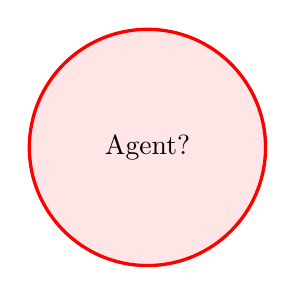
\begin{tikzpicture}
            \node[circle, draw=red, fill=red!10, very thick, minimum size=3cm] {Agent?};
        \end{tikzpicture}
        \\
        (Imagine a robot falling over and getting up again)
    \end{columns}
\end{frame}

\begin{frame}
    \frametitle{What is Reinforcement Learning?}
    \begin{itemize}
        \item \textbf{Reinforcement Learning (RL)} is a computational approach to learning from interaction.
        \item \textbf{Goal:} Maximize a numerical reward signal over time.
        \item \textbf{Key Difference:} The agent is \textbf{not} told which action to take, but must discover which actions yield the most reward by trying them.
    \end{itemize}
\end{frame}

\begin{frame}
    \frametitle{The Agent-Environment Loop}
    \centering
    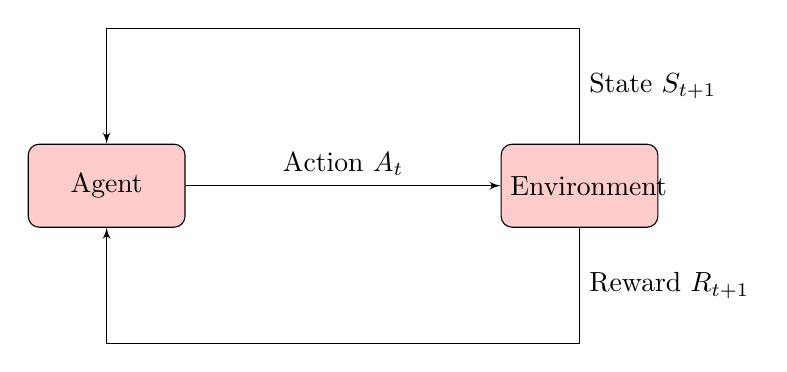
\begin{tikzpicture}[node distance = 2cm, auto]
        % Nodes
        \node [block] (agent) {Agent};
        \node [block, right=4cm of agent] (env) {Environment};

        % Lines
        \path [line] (agent) -- node {Action $A_t$} (env);
        \path [line] (env) |- node [near start] {Reward $R_{t+1}$} (2, -2) -| (agent);
        \path [line] (env) |- node [near start, swap] {State $S_{t+1}$} (2, 2) -| (agent);
    \end{tikzpicture}
    \vspace{0.5cm}

    The Agent interacts with the Environment at discrete time steps $t$.
\end{frame}

\begin{frame}
    \frametitle{Key Terminology}
    \begin{itemize}
        \item \textbf{Agent:} The learner and decision maker.
        \item \textbf{Environment:} Everything outside the agent.
        \item \textbf{Action ($A$):} What the agent does (e.g., Move Left).
        \item \textbf{State ($S$):} The current situation (e.g., Board position).
        \item \textbf{Reward ($R$):} Immediate feedback signal (Scalar).
    \end{itemize}
\end{frame}

\begin{frame}
    \frametitle{The Reward Hypothesis}
    \begin{block}{Sutton \& Barto says:}
        "That all of what we mean by goals and purposes can be well thought of as the maximization of the expected value of the cumulative sum of a received scalar signal (called reward)."
    \end{block}
    \vspace{0.5cm}
    \textbf{Example: Chess}
    \begin{itemize}
        \item Win: +1
        \item Lose: -1
        \item Draw/Intermediate moves: 0
    \end{itemize}
\end{frame}

\begin{frame}
    \frametitle{Question Time!}
    \begin{alertblock}{Scenario: Dog Training}
        You are teaching your dog to sit. You say "Sit", and if it sits, you give it a treat.
    \end{alertblock}
    \pause
    \begin{itemize}
        \item \textbf{Q:} Who is the Agent? \pause \textbf{The Dog.}
        \item \textbf{Q:} What is the Environment? \pause \textbf{You / The Room.}
        \item \textbf{Q:} What is the Reward? \pause \textbf{The Treat / "Good Boy".}
        \item \textbf{Q:} What is the Action? \pause \textbf{Sitting / Barking / Jumping.}
    \end{itemize}
\end{frame}

% -----------------------------------------------------------------------------
% Section 2: Context
% -----------------------------------------------------------------------------
\section{Context: RL vs The World}

\begin{frame}
    \frametitle{Where does RL fit?}
    The AI Landscape:
    \vspace{0.5cm}
    \begin{itemize}
        \item \textbf{Supervised Learning:} Learning with a teacher (Labels provided).
        \begin{itemize}
            \item Input: Image $\rightarrow$ Output: "Cat" (Correct!)
        \end{itemize}
        \item \textbf{Unsupervised Learning:} Finding hidden structure (Clustering).
        \begin{itemize}
            \item Input: Customer Data $\rightarrow$ Output: Segments.
        \end{itemize}
        \item \textbf{Reinforcement Learning:} Learning by interaction.
        \begin{itemize}
            \item Input: State $\rightarrow$ Action $\rightarrow$ Reward?
        \end{itemize}
    \end{itemize}
\end{frame}

\begin{frame}
    \frametitle{RL vs Supervised Learning}
    \begin{columns}
        \column{0.5\textwidth}
        \textbf{Supervised}
        \begin{itemize}
            \item Instructional feedback.
            \item "This is a cat."
            \item Independent data points.
        \end{itemize}

        \column{0.5\textwidth}
        \textbf{Reinforcement}
        \begin{itemize}
            \item Evaluative feedback.
            \item "That was good/bad (+10/-10)."
            \item Time matters (Sequential data).
            \item Feedback is often delayed.
        \end{itemize}
    \end{columns}
\end{frame}

\begin{frame}
    \frametitle{RL vs Search Algorithms (Our Course)}
    We learned about \textbf{A*}, \textbf{BFS}, \textbf{DFS}. How is RL different?
    \vspace{0.5cm}
    \begin{itemize}
        \item \textbf{Search (e.g., A*):}
        \begin{itemize}
            \item Requires a \textbf{Model} (We know the map, the rules, the costs).
            \item \textbf{Offline Planning:} The agent "thinks" before it acts to find the path.
        \end{itemize}
        \item \textbf{Reinforcement Learning:}
        \begin{itemize}
            \item Often \textbf{Model-Free} (We don't know the map initially).
            \item \textbf{Online Learning:} The agent learns the map/strategy by walking around and bumping into walls.
        \end{itemize}
    \end{itemize}
\end{frame}

\begin{frame}
    \frametitle{Comparison Table}
    \begin{center}
    \begin{tabular}{lcc}
        \toprule
        \textbf{Feature} & \textbf{Search (A*)} & \textbf{RL (Q-Learning)} \\
        \midrule
        Planning & Offline (Before acting) & Online (While acting) \\
        Model of World & Required & Not Required (Usually) \\
        Knowledge Source & Given Rules & Interaction/Experience \\
        Output & A Path & A Policy (Strategy) \\
        \bottomrule
    \end{tabular}
    \end{center}
\end{frame}

\begin{frame}
    \frametitle{BONUS: Can RL Plan?}
    \textbf{Yes! Model-Based RL.}
    \vspace{0.5cm}
    \begin{itemize}
        \item Algorithms like \textbf{AlphaZero} combine RL with Search (MCTS - Monte Carlo Tree Search).
        \item The agent learns a model of the world, then plans inside its head using that model.
    \end{itemize}
\end{frame}

\begin{frame}
    \frametitle{Question Time!}
    \begin{alertblock}{Question}
        Is A* an RL algorithm?
    \end{alertblock}
    \pause
    \textbf{No.}
    \begin{itemize}
        \item A* finds the optimal path given a graph. It doesn't "learn" a policy from scratch via rewards over time.
    \end{itemize}
\end{frame}

% -----------------------------------------------------------------------------
% Section 3: Fundamentals
% -----------------------------------------------------------------------------
\section{Fundamentals}

\begin{frame}
    \frametitle{The k-Armed Bandit Problem}
    Imagine you are in a casino with $k$ slot machines (bandits).
    \begin{itemize}
        \item Each machine pays out with a different (unknown) probability.
        \item You have $N$ coins (turns).
        \item \textbf{Goal:} Maximize your total winnings.
    \end{itemize}
    \centering
    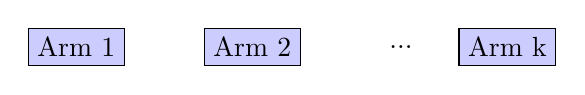
\begin{tikzpicture}
        \node[draw, fill=blue!20] (m1) {Arm 1};
        \node[draw, fill=blue!20, right=1cm of m1] (m2) {Arm 2};
        \node[right=1cm of m2] {...};
        \node[draw, fill=blue!20, right=1cm of m2, xshift=1cm] (mk) {Arm k};
    \end{tikzpicture}
\end{frame}

\begin{frame}
    \frametitle{Exploration vs Exploitation}
    This is the \textbf{core dilemma} of RL.
    \vspace{0.5cm}
    \begin{columns}
        \column{0.5\textwidth}
        \textbf{Exploitation}
        \begin{itemize}
            \item Pull the arm you \textit{think} is best.
            \item Maximize immediate reward.
            \item Risk: You might be stuck on a sub-optimal arm.
        \end{itemize}

        \column{0.5\textwidth}
        \textbf{Exploration}
        \begin{itemize}
            \item Pull a random arm / unknown arm.
            \item Gather information.
            \item Risk: You might lose money now to gain knowledge for later.
        \end{itemize}
    \end{columns}
\end{frame}

\begin{frame}
    \frametitle{A Simple Solution: $\epsilon$-Greedy}
    How do we balance this?
    \begin{block}{$\epsilon$-Greedy Algorithm}
        Before every action, flip a biased coin:
        \begin{itemize}
            \item With probability $1 - \epsilon$: \textbf{Exploit} (Choose best known action).
            \item With probability $\epsilon$: \textbf{Explore} (Choose random action).
        \end{itemize}
    \end{block}
    Usually, $\epsilon$ is small (e.g., 0.1) and decays over time.
\end{frame}

\begin{frame}
    \frametitle{From Bandits to Context}
    Bandits have only \textbf{one state}.
    \begin{itemize}
        \item Life involves sequences.
        \item Your action now affects your position tomorrow.
    \end{itemize}
    \textbf{Enter: Markov Decision Processes (MDPs).}
\end{frame}

\begin{frame}
    \frametitle{The Markov Property}
    \begin{block}{Definition}
        "The future depends only on the present, not the past."
    \end{block}
    \vspace{0.5cm}
    $$P(S_{t+1} | S_t, A_t)$$
    covers everything we need.
    \begin{itemize}
        \item Example: A Chess board position.
        \item You don't need to know the history of moves to decide the next best move. The physics of the game is fully contained in the current board configuration.
    \end{itemize}
\end{frame}

\begin{frame}
    \frametitle{Components of an MDP}
    An MDP is defined by a tuple $(\mathcal{S}, \mathcal{A}, \mathcal{P}, \mathcal{R}, \gamma)$:
    \begin{enumerate}
        \item \textbf{States ($\mathcal{S}$):} All possible situations.
        \item \textbf{Actions ($\mathcal{A}$):} All possible things to do.
        \item \textbf{Transition Probability ($\mathcal{P}$):} Physics of the world. If I jump, do I land or fall?
        \item \textbf{Reward Function ($\mathcal{R}$):} The goal.
        \item \textbf{Discount Factor ($\gamma$):} How much we care about the future.
    \end{enumerate}
\end{frame}

\begin{frame}
    \frametitle{The Discount Factor ($\gamma$)}
    Why do we discount future rewards? ($\gamma \in [0, 1]$)
    \begin{itemize}
        \item \textbf{Mathematical:} Keeps the sum of infinite rewards finite.
        \item \textbf{Uncertainty:} The future is uncertain. A treat now is better than a promised treat next year.
        \item \textbf{$\gamma = 0$:} Myopic Agent (Only cares about immediate reward).
        \item \textbf{$\gamma \to 1$:} Far-sighted Agent.
    \end{itemize}
\end{frame}

\begin{frame}
    \frametitle{Policies and Value Functions}
    \begin{itemize}
        \item \textbf{Policy ($\pi$):} The Agent's Brain.
        $$ \pi(a|s) = P(A_t=a | S_t=s) $$
        Mapping from state to action. "If I see X, I do Y".

        \item \textbf{Value Function ($V(s)$):}
        "How good is it to be in this state?"
        $$ V_\pi(s) = \mathbb{E}[R_{t+1} + \gamma R_{t+2} + \dots | S_t = s] $$
    \end{itemize}
\end{frame}

\begin{frame}
    \frametitle{Value Function Intuition}
    \centering
    \textbf{Tic-Tac-Toe}
    \vspace{0.5cm}

    \begin{itemize}
        \item State A: You have two Xs in a row. \textbf{High Value.}
        \item State B: Opponent has two Os in a row. \textbf{Low Value.}
    \end{itemize}

    The value function predicts the eventual outcome.
\end{frame}

\begin{frame}
    \frametitle{Action-Value Functions ($Q(s, a)$)}
    Often we want to know: "How good is it to take action $A$ in state $S$?"
    \vspace{0.5cm}
    \begin{itemize}
        \item This is denoted as $Q(s, a)$.
        \item If we know the optimal $Q^*(s, a)$ for all actions, the optimal policy is easy:
        $$ \pi^*(s) = \arg\max_a Q^*(s, a) $$
        \item Just pick the action with the highest Q-value!
    \end{itemize}
\end{frame}

\begin{frame}
    \frametitle{Tabular Q-Learning}
    Imagine a giant Excel sheet (Table).
    \begin{itemize}
        \item Rows = All possible States.
        \item Columns = All possible Actions.
        \item Cells = The Q-value (Expected future reward).
    \end{itemize}

    \begin{center}
    \begin{tabular}{|c|c|c|c|}
    \hline
     & \textbf{Left} & \textbf{Right} & \textbf{Jump} \\
    \hline
    State 1 & 0.5 & 2.0 & -1.0 \\
    \hline
    State 2 & 1.1 & 0.1 & 5.0 \\
    \hline
    ... & ... & ... & ... \\
    \hline
    \end{tabular}
    \end{center}

    We update these numbers as we explore the world.
\end{frame}

\begin{frame}
    \frametitle{Question Time!}
    \begin{alertblock}{Problem}
        Why can't we use a table (Excel sheet) for a self-driving car?
    \end{alertblock}
    \pause
    \textbf{Too many states!}
    \begin{itemize}
        \item The car sees a camera feed.
        \item Pixel values are continuous.
        \item Position is continuous.
        \item You cannot list every possible millisecond of driving as a row in a table.
    \end{itemize}
\end{frame}

% -----------------------------------------------------------------------------
% Section 4: Deep RL
% -----------------------------------------------------------------------------
\section{Deep RL}

\begin{frame}
    \frametitle{The Curse of Dimensionality}
    \begin{itemize}
        \item \textbf{Tic-Tac-Toe:} ~5,000 states. (Table works).
        \item \textbf{Chess:} $10^{47}$ states. (Table impossible).
        \item \textbf{Go:} $10^{170}$ states. (More than atoms in universe).
        \item \textbf{Real World Images:} $256^{100 \times 100}$ ...
    \end{itemize}
    We need a better way.
\end{frame}

\begin{frame}
    \frametitle{Solution: Function Approximation}
    Instead of \textbf{memorizing} every state, we want to \textbf{generalize}.
    \vspace{0.5cm}
    \begin{itemize}
        \item If State A looks like State B, the value should be similar.
        \item We approximate the Q-table with a function:
        $$ Q(s, a) \approx f(s, a, \theta) $$
    \end{itemize}
\end{frame}

\begin{frame}
    \frametitle{Enter Neural Networks (Deep Q-Networks)}
    We use a \textbf{Neural Network} to approximate the Q-function.
    \vspace{0.5cm}
    \begin{center}
    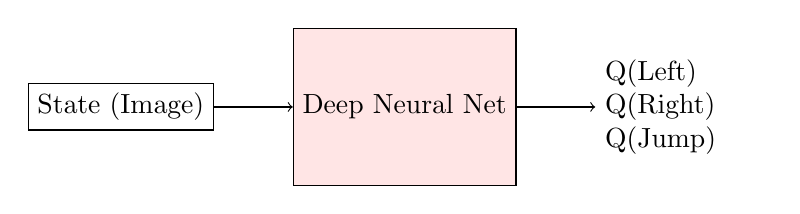
\begin{tikzpicture}
        \node[draw] (input) {State (Image)};
        \node[right=1cm of input, draw, fill=red!10, minimum height=2cm] (nn) {Deep Neural Net};
        \node[right=1cm of nn, text width=2cm] (output) {Q(Left)\\Q(Right)\\Q(Jump)};
        \draw[->] (input) -- (nn);
        \draw[->] (nn) -- (output);
    \end{tikzpicture}
    \end{center}
    The weights $\theta$ of the network replace the table entries.
\end{frame}

\begin{frame}
    \frametitle{Connecting to CNNs}
    You already know Convolutional Neural Networks (CNNs)!
    \begin{itemize}
        \item For Atari games, the input is raw pixels.
        \item We use CNN layers to extract features (edges, shapes, objects).
        \item These features are fed into dense layers to output Action Values.
    \end{itemize}
\end{frame}

\begin{frame}
    \frametitle{Deep RL Challenges}
    Sounds easy? It's not.
    \begin{itemize}
        \item \textbf{Unstable:} RL with NNs is notoriously unstable.
        \item \textbf{Moving Target:} In Supervised Learning, the target (label) is fixed. In RL, our target (estimated Q) keeps changing as we learn.
        \item \textbf{Correlated Data:} Sequential video frames are highly correlated. NNs assume independent data (i.i.d).
    \end{itemize}
\end{frame}

\begin{frame}
    \frametitle{BONUS: Experience Replay}
    How DQN solved the correlation problem:
    \begin{block}{Experience Replay Buffer}
        \begin{enumerate}
            \item As the agent plays, save experiences $(S, A, R, S')$ into a large memory buffer.
            \item To train, sample a \textbf{random batch} from this memory.
        \end{enumerate}
    \end{block}
    This breaks the correlation between consecutive frames and stabilizes training.
\end{frame}

\begin{frame}
    \frametitle{Alternative: Policy Gradients}
    \begin{itemize}
        \item DQN is \textbf{Value-Based} (learns Q-values).
        \item \textbf{Policy-Based} methods learn the Policy $\pi$ directly.
        \item They adjust the probability of taking actions.
        \item If Action A led to good reward $\rightarrow$ Increase $P(A)$.
        \item Popular Algorithms: REINFORCE, \textbf{PPO} (Proximal Policy Optimization).
    \end{itemize}
\end{frame}

\begin{frame}
    \frametitle{Family Tree of RL}
    \begin{itemize}
        \item \textbf{Model-Free}
        \begin{itemize}
            \item Value-Based (DQN, Double DQN)
            \item Policy-Based (REINFORCE)
            \item Actor-Critic (A2C, PPO, SAC)
        \end{itemize}
        \item \textbf{Model-Based}
        \begin{itemize}
            \item AlphaZero (MCTS + RL)
            \item World Models
        \end{itemize}
    \end{itemize}
\end{frame}

% -----------------------------------------------------------------------------
% Section 5: Tools & History
% -----------------------------------------------------------------------------
\section{Tools \& History}

\begin{frame}
    \frametitle{History: Atari 2600}
    \begin{itemize}
        \item \textbf{2013:} DeepMind introduced DQN.
        \item First agent to play generic Atari games at human level directly from pixels.
        \item Before this, RL relied on hand-crafted features tailored for each game.
        \item This sparked the "Deep RL" revolution.
    \end{itemize}
\end{frame}

\begin{frame}
    \frametitle{The Environment Standard}
    To compare algorithms, we need standard benchmarks.
    \vspace{0.5cm}
    \begin{itemize}
        \item \textbf{OpenAI Gym} (now maintained as \textbf{Gymnasium}).
        \item Provides a standard API for environments.
        \item Allows swapping environments with one line of code.
    \end{itemize}
\end{frame}

\begin{frame}[fragile]
    \frametitle{The Gym API}
    \begin{lstlisting}
import gymnasium as gym

env = gym.make("CartPole-v1")
observation, info = env.reset()

for _ in range(1000):
    # Sample random action
    action = env.action_space.sample()

    # Step the environment
    obs, reward, terminated, truncated, info = env.step(action)

    if terminated or truncated:
        observation, info = env.reset()
    \end{lstlisting}
\end{frame}

\begin{frame}
    \frametitle{Standard Benchmarks}
    \begin{enumerate}
        \item \textbf{Classic Control:} CartPole, MountainCar (Simple physics).
        \item \textbf{Atari:} Breakout, Pong, Space Invaders (Pixel input).
        \item \textbf{MuJoCo:} Continuous control for robotics (Walking, hopping).
    \end{enumerate}
\end{frame}

\begin{frame}
    \frametitle{Action Spaces}
    Important distinction when choosing algorithms:
    \vspace{0.5cm}
    \begin{itemize}
        \item \textbf{Discrete Space:} Finite set of actions.
        \begin{itemize}
            \item [Left, Right, Jump]
            \item Example: Super Mario, Atari.
        \end{itemize}
        \item \textbf{Continuous Space:} Real-valued vectors.
        \begin{itemize}
            \item [Steering Angle 23.4, Gas Pedal 0.8]
            \item Example: Robotics, Self-driving cars.
        \end{itemize}
    \end{itemize}
\end{frame}

\begin{frame}
    \frametitle{Question Time!}
    \begin{alertblock}{Question}
        In Flappy Bird, is the action space Discrete or Continuous?
    \end{alertblock}
    \pause
    \textbf{Discrete.}
    \begin{itemize}
        \item You either \textbf{Flap} or you \textbf{Don't Flap}.
        \item Binary action space $\{0, 1\}$.
    \end{itemize}
\end{frame}

% -----------------------------------------------------------------------------
% Section 6: Hands-on Flappy Bird
% -----------------------------------------------------------------------------
\section{Project: Flappy Bird Agent}

\begin{frame}
    \frametitle{Let's Build an Agent!}
    \textbf{Objective:} Teach an AI to play Flappy Bird.
    \vspace{0.5cm}
    \begin{itemize}
        \item We will use the `flappy-bird-gymnasium` library.
        \item We will use `Stable Baselines3` (PPO algorithm).
    \end{itemize}
\end{frame}

\begin{frame}
    \frametitle{State Representation}
    What does the agent see?
    \begin{itemize}
        \item We \textit{could} use raw pixels (CNN), but training takes longer.
        \item For this workshop, we use \textbf{extracted coordinates}.
    \end{itemize}
    \vspace{0.5cm}
    \textbf{State Vector (12 dimensions):}
    \begin{itemize}
        \item Horizontal distance to next pipe.
        \item Vertical distance to next pipe.
        \item Player vertical velocity.
        \item ...
    \end{itemize}
\end{frame}

\begin{frame}
    \frametitle{Designing the Reward}
    We need to tell the agent what we want.
    \begin{itemize}
        \item \textbf{Alive:} +0.1 per frame. (Encourage survival).
        \item \textbf{Pass Pipe:} +1.0. (Encourage progress).
        \item \textbf{Death:} -100.0 or just Game Over. (Discourage crashing).
    \end{itemize}
\end{frame}

\begin{frame}
    \frametitle{Choosing the Algorithm}
    We chose \textbf{PPO (Proximal Policy Optimization)}.
    \begin{itemize}
        \item It is the state-of-the-art for many tasks.
        \item Reliable and easy to tune compared to DQN.
        \item Available in Stable Baselines3.
    \end{itemize}
\end{frame}

\begin{frame}[fragile]
    \frametitle{The Code}
    \begin{lstlisting}
import gymnasium as gym
import flappy_bird_gymnasium
from stable_baselines3 import PPO

# 1. Create Environment
env = gym.make("FlappyBird-v0")

# 2. Define Model (PPO)
model = PPO("MlpPolicy", env, verbose=1)

# 3. Train
model.learn(total_timesteps=100000)

# 4. Save
model.save("flappy_bird_expert")
    \end{lstlisting}
\end{frame}

\begin{frame}
    \frametitle{LIVE DEMO}
    \begin{center}
        \Huge \textbf{DEMO TIME}
        \vspace{1cm}

        \large
        1. Watch untrained agent (Random flailing).\\
        2. Watch trained agent (God Mode).
    \end{center}
\end{frame}

% -----------------------------------------------------------------------------
% Section 7: Applications & Conclusion
% -----------------------------------------------------------------------------
\section{Applications \& Conclusion}

\begin{frame}
    \frametitle{RL is Everywhere}
    It's not just about video games anymore.
    \begin{itemize}
        \item Robotics
        \item Language Models (LLMs)
        \item Industrial Control
        \item Autonomous Driving
    \end{itemize}
\end{frame}

\begin{frame}
    \frametitle{Robotics}
    \textbf{Sim-to-Real Transfer}
    \begin{itemize}
        \item Training a robot in the real world is slow and dangerous (it falls and breaks).
        \item We train in a physics simulator (MuJoCo/Isaac Gym) using RL.
        \item We transfer the "brain" to the real robot.
        \item Example: Boston Dynamics, ANYbotics.
    \end{itemize}
\end{frame}

\begin{frame}
    \frametitle{LLMs and RLHF}
    \textbf{ChatGPT / Claude / Gemini}
    \begin{itemize}
        \item Large Language Models are first trained to predict the next word (Supervised).
        \item Then they are fine-tuned using \textbf{RL from Human Feedback (RLHF)}.
        \item Humans rate the answers (Reward Model).
        \item PPO is used to optimize the LLM to generate high-reward answers (Helpful, Honest, Harmless).
    \end{itemize}
\end{frame}

\begin{frame}
    \frametitle{Industrial Applications}
    \textbf{Google Data Centers}
    \begin{itemize}
        \item DeepMind used RL to control cooling fans and windows in Google data centers.
        \item Reduced cooling energy bill by \textbf{40\%}.
        \item Action: Adjust fan speed. Reward: -Energy Usage.
    \end{itemize}
\end{frame}

\begin{frame}
    \frametitle{Summary}
    \begin{enumerate}
        \item \textbf{RL} is learning by interaction (Action, State, Reward).
        \item \textbf{Exploration vs Exploitation} is the key trade-off.
        \item \textbf{MDPs} provide the mathematical framework.
        \item \textbf{Deep RL} (DQN, PPO) scales RL to complex worlds using Neural Networks.
        \item \textbf{Applications} range from Atari to Robotics to ChatGPT.
    \end{enumerate}
\end{frame}

\begin{frame}
    \frametitle{Resources}
    \textbf{Want to learn more?}
    \begin{itemize}
        \item \textbf{Book:} \textit{Reinforcement Learning: An Introduction} (Sutton \& Barto).
        \item \textbf{Course:} Hugging Face Deep RL Course (Free, Online).
        \item \textbf{Library:} Stable Baselines3 (Python).
    \end{itemize}
\end{frame}

\begin{frame}
    \frametitle{Thank You!}
    \begin{center}
        \Huge \textbf{Questions?}
        \vspace{1cm}

        \large
        (Bonus points for hard questions!)
    \end{center}
\end{frame}

\end{document}
